\documentclass[hyperref={pdfpagelayout=SinglePage}]{beamer}
\mode<presentation> {
\usetheme{Berlin}

\setbeamertemplate{footline}[page number] 
\setbeamertemplate{navigation symbols}{} 
\setbeamertemplate{itemize item}[square]
\setbeamertemplate{itemize subitem}[circle]
\setbeamertemplate{itemize subsubitem}[default]
}
\usepackage{graphicx}
\usepackage{verbatim}
\usepackage{smartdiagram}
\usepackage{minted}
\usepackage{multicol}
\setlength{\columnsep}{1cm}
\newenvironment{mysubsec}[1]
{   \begin{frame}
	\frametitle{#1} }
{ \end{frame} }
%----------------------------------------------------------------------------------------
%   TITLE PAGE
%----------------------------------------------------------------------------------------
\title{A Dataflow Approach to the ROS Architecture}
\author{Orestis Melkonian} 
\institute[UoA]
{
	Software \& Knowledge Engineering Laboratory (SKEL)\\
	\medskip
	\textit{o.melkonian@di.uoa.gr} 
}
\date{\today}
\begin{document}
\begin{frame}
	\titlepage
\end{frame}

\begin{frame} \frametitle{Overview}
	\tableofcontents
\end{frame}
%----------------------------------------------------------------------------------------
\section{Introduction}
	\begin{frame} \frametitle{Introduction}
		\begin{center}		
		\smartdiagramset{set color list={orange!60, green!50!lime!60,blue!20!black!30!green,
		blue!50!cyan},
		uniform connection color=true,
		bubble center node size=1,
		bubble node size=1
		}
		\smartdiagram[bubble diagram]{Robotics,
		  Computer\\Science, Mechanical\\Engineering, Electrical\\Engineering, Cognitive\\Science, Web\\Development}
		\end{center}
	\end{frame}
	\begin{mysubsec}{Future}  
		\begin{itemize}
		\item Ubiquitous Robotic Systems
		\item Web Robotics
		\item Minimum-cost robotics research
		\item Rapid prototyping
		\end{itemize}
	\end{mysubsec}	
%------------------------------------------------------------------
\section{Motivation}
	\begin{frame} \frametitle{Motivation}
		\begin{itemize}
		\item Satisfied with current languages on ROS?
		\item Right amount of abstraction?
		\item Logical perspective in sync with code we write?
		\item Real-time systems
			\begin{itemize} \item Do existing languages provide time modelling? \end{itemize}
		\item Continuous streams of data
			\begin{itemize} \item Do existing languages provide appropriate stream handling? \end{itemize}
		\item Too much technicalities that are not part of the main problem
			\begin{itemize} \item Maybe a compiler can do them automatically \end{itemize}			
		\item Do problems faced in robotics have a dataflow nature?
			\begin{itemize} \item If so, why not code in a dataflow language? \end{itemize}			
		\end{itemize}
	\end{frame}
%------------------------------------------------------------------
 \section{Example}
	\begin{frame}[allowframebreaks] \frametitle{Example}
		\begin{multicols*}{2}
		[\center \textbf{A drone progressing in a hall}]
		\begin{itemize}
		\item 4 sonar sensors {\footnotesize (UP,DOWN,LEFT,RIGHT)}
		\item Default move: {\footnotesize AHEAD}
		\item Depending on sensor data, change direction to avoid collision with any of the four walls
		\item Also occasional sonar sensor malfunction (negative values)
		\end{itemize}		
		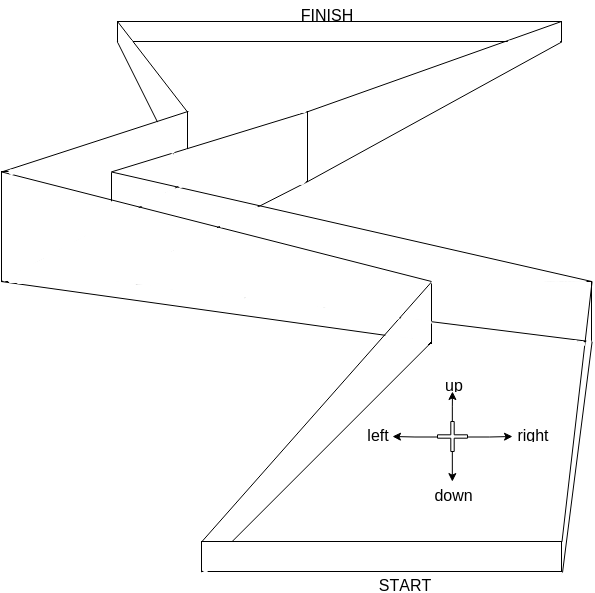
\includegraphics[scale=0.25,keepaspectratio]{pics/Drone-hall.png}
		\end{multicols*}
	\framebreak
		\inputminted[fontsize=\tiny]{cpp}{code/example/imper.cpp}
	\framebreak
		\inputminted[fontsize=\tiny]{hs}{code/example/flow.hs}
		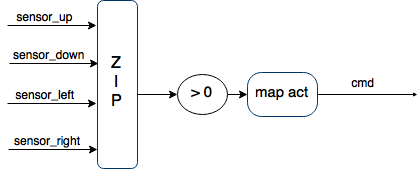
\includegraphics[scale=0.35,keepaspectratio]{pics/example.png}
	\end{frame}	
%------------------------------------------------------------------
\section{Another Example}
	\begin{frame} \frametitle{Another Example}
		\begin{multicols*}{2}
		[ \center \textbf{Implementation of a PID controller} ]
		\inputminted[fontsize=\tiny]{hs}{code/pid/pid.hs}
		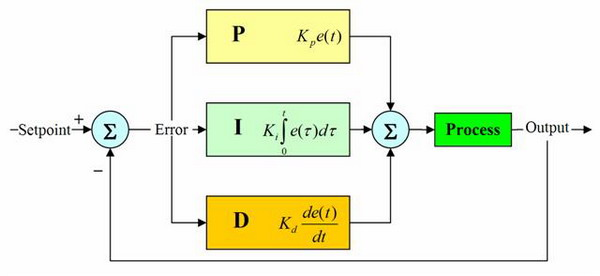
\includegraphics[scale=0.25,keepaspectratio]{pics/pid.jpg}
		\end{multicols*}		
	\end{frame}	
%------------------------------------------------------------------	
\section{Problems}
	\begin{frame}[allowframebreaks] \frametitle{Problems}
		\begin{itemize}
		\item \textbf{Scalability}
			\begin{itemize}
			\item Asynchronous behaviour using callback functions
			\item Complex schemes require "internal plumbing"
			\item Unreadable, difficult to maintain
			\item Does not separate data from control
			\end{itemize}
		\item \textbf{Untyped topics}
			\begin{itemize}
			\item Topics are just named pipes
			\item No type-safety
			\item Hard to impose constraints on them
			\item e.g. Visual detection on audio streams
				\begin{itemize}
				\item Does not catch errors at compile time
				\end{itemize}
			\end{itemize}	
		\framebreak	
		\item \textbf{Time modelling}
			\begin{itemize}
			\item Control theory models robot behaviour primarily using differential equations on time
			\item Existing languages do not provide the concept of time
			\item Need to implement tedious delta timing
			\item But why? Time is logical
			\item Need to have temporal nature by design
			\end{itemize}
		\item \textbf{Compiler restriction}
			\begin{itemize}
			\item Coder explicitly specifies where nodes are being executed
			\item Won't allow intelligent runtime re-configurations 
			\\ e.g. for optimal power management, minimum execution time
			\end{itemize}
		\framebreak
		\item \textbf{Verifiability} 
			\begin{itemize}
			\item Robots are becoming an integral part of our everyday life
			\item More and more responsibility
			\\ e.g. babysitters, security monitoring, space robots
			\item Must be able to prove program correctness
			\item Nearly impossible for low-level languages
			\item Need for more precise semantics
			\end{itemize}
%		\item \textbf{Concurrency}
%			\begin{itemize}
%			\item Actor model provides coarse-grained parallelism 
%			\begin{itemize} \item Nodes as actors \end{itemize}
%			\item But we also need fine-grained parallelism
%			\begin{itemize} \item Multi-threaded nodes \end{itemize}
%			\item Code inside code full of side-effects, shared states, fragile synchronization
%			\item Difficult to automatically make parallel
%			\\ e.g. C pointers $\rightarrow$ No guarantee for memory location
%			\end{itemize}
%		\framebreak
%		\item \textbf{Advanced cognitive functions}
%			\begin{itemize}
%			\item We must catch up with robot capabilities
%			\item Higher-level cognitive functions should be programmed in an appropriate language
%			\\ e.g. Reasoning
%			\end{itemize}
%		\item \textbf{Web technology utilization}	
%			\begin{itemize}
%			\item Endless possibilities appearing in Web Robotics
%			\item We can access the web using \textit{rosbridge} and \textit{rosjs}, but...
%			\item It's a streaming world!
%			\item So efficient stream processing capabilities are mandatory
%			\end{itemize}
		\end{itemize}
	\end{frame}
%------------------------------------------------------------------
\section{Solutions}
	\begin{frame}[allowframebreaks] \frametitle{Solutions}
		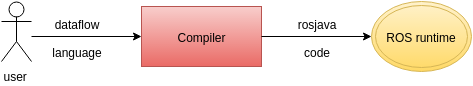
\includegraphics[scale=0.65]{pics/model.png}
		\begin{itemize}
		\item \textbf{A domain-specific dataflow language}
			\begin{itemize}
			\item ROS architecture essentially defines a dataflow graph	\\
			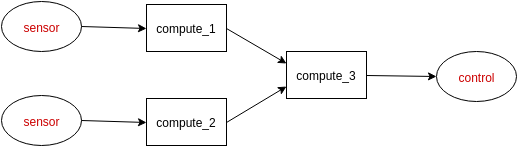
\includegraphics[scale=0.4]{pics/ros_dataflow.png}
			\item Composable stream-processing operators \\ 
			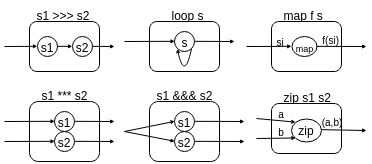
\includegraphics[scale=0.7]{pics/streams.png}
			\framebreak
			\item Timely model $\rightarrow$ Simpler, portable code	\\
			e.g. \\
			\hspace{20pt} $x(t) = 1/2 \int_{0}^{t}(u_l(t)+u_r(t))cos\theta(t)dt$ \\
			\hspace{60pt} $\Downarrow$ \\
			\inputminted[fontsize=\scriptsize]{hs}{code/time.hs}
			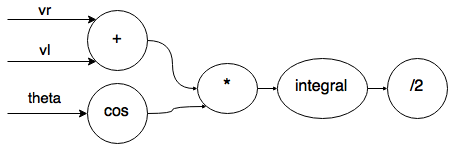
\includegraphics[scale=0.5]{pics/time.png} 
			\framebreak
			\item Separates data from control \\
			\inputminted[fontsize=\scriptsize]{cpp}{code/control-data/imper.cpp}
			\hspace{60pt} $\Downarrow$ \\
			\inputminted[fontsize=\scriptsize]{hs}{code/control-data/flow.hs}		
			\end{itemize}
			\framebreak
		\item \textbf{Topics as streams}
			\begin{itemize}
			\item First-class citizens
			\item At last, type-safety!
			\inputminted[fontsize=\scriptsize]{hs}{code/typed_stream.hs}
			\item Automatic \textit{rosmsg} generation
			\item We now can catch errors at compile time
			\end{itemize}
		\item \textbf{Pure functions to the rescue}
			\begin{itemize}
			\item Keep maximum portion of the program as pure functions
			\item No side-effects $\rightarrow$ equational reasoning
			\item Can prove program correctness
			\end{itemize}
		\framebreak		
		\item \textbf{Dynamic reconfiguration}
			\begin{itemize}
			\item Locality-agnostic node execution
			\item System will allocate nodes to machines for optimality
			\item Ability to specify preferences \\ e.g. run 'graph' --powersave/--uniform /--mintime
			\end{itemize}
%		\item \textbf{Dataflow analysis}
%			\begin{itemize}
%			\item Huge body of research on the dataflow computation model
%			\item Starting as early as 1974 with Kahn's process networks
%			\item Encourages parallelism
%			\item Suitable for real-time systems
%			\item Dataflow representation enables rule-based optimization techniques
%			\\ e.g. Datalog program recognizing proper transformations based on logical relations
%			\end{itemize}			
%		\framebreak	
		\item \textbf{Harness the cloud!}
			\begin{itemize}
			\item Adopt the advantages of web-based solutions to develop robotic applications
			\item Use the cloud to get access to distributed computing resources \\ e.g. Grasping using the Google Object Recognition Engine
			\end{itemize}
%		\item \textbf{Stream reasoning}
%			\begin{itemize}
%			\item Draw from Semantic Data research
%			\item Reason about rapidly changing data	
%			\item Enable rapid development of advanced cognitive functions
%			\end{itemize}
		\end{itemize}			
	\end{frame}
%------------------------------------------------------------------
\section{Related Work}		
	\begin{mysubsec}{Functional Reactive Programming (FRP)}
		\begin{itemize}
		\item A programming paradigm suitable for hybrid systems
		\item Uses the building blocks of functional programming
		\\ (\textit{map,filter,...})
		\item For systems that are:
			\begin{itemize}
			\item Responsive
			\item Resilient	
			\item Elastic
			\item Message-driven
			\end{itemize}
		\item Explicit time modelling
		\item Express event-handling in a natural way
		\item Applications in GUIs, robotics and music.
		\end{itemize}
	\end{mysubsec}
	\begin{mysubsec}{Robotics}
		\begin{itemize}
		\item \textbf{roshask}
			\begin{itemize}
			\item A Haskell-binding client library for ROS
			\item Takes the first step towards stream-oriented robotics
			\item Implements topics as first-class citizens
			\item Provides some basic stream manipulation
			\end{itemize}
		\item \textbf{Frob}
			\begin{itemize}
			\item A domain-specific language (DSL)
			\item Realization of the FRP model on robotics
			\item Complex robot behaviours in a few lines of code
			\item Implementation exists in Haskell (Yampa)
			\item Several performance issues (time-/space-leaks)
			\end{itemize}			
		\end{itemize}
	\end{mysubsec}
	\begin{mysubsec}{Big Data}
		\begin{itemize}
		\item \textbf{Akka}
			\begin{itemize}
			\item A framework for scalable, distributed, message-driven applications
			\item Incorporates the Actor model, like ROS
			\item The stream handling seemed to be error-prone and tedious
			\item The inability to treat streams efficiently and intuitively led them to develop the Akka Streams API
			\item Also influenced by FRP
			\end{itemize}
		\framebreak
		\item \textbf{Naiad}
			\begin{itemize}
			\item A distributed system for cyclic parallel dataflow programming
			\item A new computational model: \textit{Timely dataflow}
			\item Many novel approaches for efficient dataflow graphs
			\end{itemize}
		\end{itemize}
	\end{mysubsec}
	\begin{mysubsec}{Ziria: A DSL for wireless systems programming}  
		\begin{itemize}
			\item Designed by Haskell-lovers
			\item Also inspired by Functional Reactive Programming (FRP)
			\item Towards Software-Defined Radios (SDR)
			\item In contrast to SORA (low-level C++ library)
			\item High-level functional language replaces low-level C
			\item Implementation of a Wifi Receiver
			\begin{itemize}
				\item SORA $\rightarrow$ 23000 lines of code
				\item Ziria $\rightarrow$ 3000 lines of code
			\end{itemize}
			\item Implementation of a Scrambler
			\begin{itemize}
				\item SORA $\rightarrow$  90 lines of code
				\item Ziria $\rightarrow$ 20 lines of code
			\end{itemize}
			\item But same performance!
		\end{itemize}	
	\end{mysubsec}	
%------------------------------------------------------------------
%\section{Technological Decisions}
%	\begin{mysubsec}{To contribute or not to contribute?}
%		\begin{itemize}
%			\item \textit{roshask} at an experimental level
%			\item integration overhead \textit{VS} reinvent-the-wheel overhead
%			\item From scratch means dealing with irrelevant technicalities
%			\\	 e.g. Setting up messages, Necessary client library API
%			\item Otherwise, build upon \textit{rosjava} possibly using Scala as the host language
%		\end{itemize}
%	\end{mysubsec}
%	\begin{mysubsec}{Which aspect to focus on?}
%		\begin{itemize}
%			\item Many opportunities from a wide range of research fields, but limited time
%			\item Must focus on the core topics, to enable meaningful future contributions
%			\begin{itemize}
%				\item Concrete language semantics
%				\item Expressiveness
%				\item Efficient implementation
%			\end{itemize}
%			\item Likely to leave out web-related features
%		\end{itemize}
%	\end{mysubsec}
%------------------------------------------------------------------
\section{Conclusion}
\begin{frame} \frametitle{Conclusion}
	\begin{itemize}	
	\item There will be some learning curve
	\item But it will pay off in terms of:
		\begin{itemize}
		\item Productivity
		\item Cleaner, safer, scalable code
		\item More efficient resource management
		\item Faster robotics research
		\end{itemize}
	\item Any DSL design relies heavily on feedback from domain experts
	\item There is a general pattern here
		\begin{itemize} \item Abstraction is the way! \end{itemize}
	\end{itemize}
\end{frame}
%------------------------------------------------------------------
\iffalse
\section{References}
\begin{frame}[allowframebreaks]
    \frametitle{References}
    \nocite{*}
    \bibliographystyle{unsrt}
	\bibliography{ref}
\end{frame}
\fi
%------------------------------------------------------------------
\begin{frame}
	\Huge{\centerline{The End}}
\end{frame}
\end{document}
